\section{The Atomic Orchid Platform}
In this section we describe the platform within which we embed the planning agent in order study the interactions between human responders and the agent and derive design guidelines for the implementation of such planning agents in real-world scenarios. (\textbf{Joel: please add justification for a mixed-reality game approach to testing this scenario v/s other approaches}). 

In more detail, AtomicOrchid is a location-based mobile game based on the fictitious scenario described in Section \ref{sec:scenario}. Field responders are assigned a specific role (e.g. `medic', `transporter', `soldier', `ambulance') 
In their mission to rescue all the targets from the radioactive zone, the field responders are supported by (at least one) person in a centrally located HQ room, and the planning agent that sends the next task (as computed in the previous section) to the team of field responders. In what follows, we first present the player interfaces used, the interactions with the planning agent, and the modelling of the radiation cloud in the game.

\subsection{Player interfaces}
Field responders are equipped with a `mobile responder tool' providing sensing and awareness capabilities in three tabs (geiger counter, map, messaging and tasks; see figure XX). One tab shows a reading of radioactivity, player health level (based on exposure), and a GPS-enabled map of the game area to locate fellow responders, the targets to be rescued and the drop off zones for the targets. Another tab provides a broadcast messaging interface to communicate with fellow responders (field responders and HQ). Another tab shows the team and task allocation dynamically provided by the agent. Notifications are used to alert both to new messages and task allocations.

The HQ is manned by at least one player who has at her disposal an `HQ dashboard' that provides an overview of the game area, including real-time information of the players' locations (see figure XX). The dashboard provides a broadcast messaging widget, and a player status widget so that the responders' exposure and health levels can be monitored. HQ can further monitor the  current team and task allocations by the agent. Importantly, only the HQ has a view of the radioactive cloud, depicted as a heatmap. `Hotter' zones correspond with higher levels of radioactivity.

\subsection{Planning agent}
[Wenchao. Describe how the agent works (not implementation detail, add that in subsection below), i.e., when it is polled, what information is being exchanged, and how the team/task allocation is being constructed from that and sent.]
\subsection{Radiation Cloud Modelling}\label{sec:radiation}
\noindent The radiation cloud is assumed to be monitored using a number of sensors on the ground (within the disaster space) that collect readings of the radiation cloud intensity and wind velocity every minute of the game. These sensors can be at fixed locations or held by mobile agents.  The radiation cloud diffusion process is modelled in a standard way by a nonlinear Markov field stochastic differential equation,  
\begin{eqnarray*}
\frac{D \text{Rad}({\bf z}, \tau)}{D \tau}=\kappa \triangledown^2 \text{Rad}({\bf z},\tau)-\text{Rad}({\bf z},\tau)\triangledown \cdot {\bf w}({\bf z},\tau)+\sigma({\bf z},\tau)
\end{eqnarray*}
where $D$ is the material derivative, $\text{Rad}({\bf z},\tau)$ is the radiation cloud intensity at location ${\bf z}$ at time $\tau$, $\kappa$ is a fixed diffusion coefficient and $\sigma$ is the radiation source(s) emission rate. The diffusion equation is solved on a regular grid defined across the environment with grid coordinates $G$ (as defined in Section \ref{sec:model}).  Furthermore, the grid is solved at discrete time instances $\tau$.  The cloud is driven by wind forces which vary both spatially and temporally.  These forces induce anisotropy into the cloud diffusion process which is proportional to the wind velocity, ${\bf w}({\bf z},\tau)$.  The wind velocity is drawn from two independent Gaussian processes (GP), one GP for each Cartesian coordinate axis, $w_i({\bf z},\tau)$, of ${\bf w}({\bf z},\tau)$.  The GP captures both the spatial distribution of the wind velocity and the dynamic process resulting from shifting wind patterns such as short term gusts and longer term variations. 

% In our simulation, each spatial wind velocity component is modelled by a squared-exponential GP covariance function, $K$, with fixed input and output scales (although any covariance function can be substituted). Furthermore, as wind conditions may change over time we introduce a temporal correlation coefficient, $\rho$, to the covariance function.  Thus, for a single component, $w_i$, of ${\bf w}$, defined over grid $G$ at times $\tau$ and $\tau^\prime$, the wind process covariance function is, $\text{Cov}(w_i(G,\tau),w_i(G,\tau^\prime))=\rho(\tau,\tau^\prime) K(G,G)$.  We note that, when $\rho=1$ the wind velocities are time invariant (although spatially variant).  Values of $\rho<1$ model wind conditions that change over time.

Using the above model, we are able to create a moving radiation cloud, thus posing a real challenge both for the HQ (agent and commander) and the responders on the ground, as predictions they can make of where the cloud will move to will be prone to uncertainty both to the simulated wind speed and direction. 


%(\textbf{Steve: in the platform we take the `real' values from the diffusion process i believe. Does the above capture this? We will say that we will add the features you mention below to a future version of the platform where we aim to do both situational awareness and rescue. Add a sentence above to conclude where we took the values from and the process takes into account the  location of radiation source. Also, your notation clashes with the notations in the scenario and Feng's algorithm - please try to align.}
%The cloud intensity and wind velocity are measured by {\it monitor agents} equipped with geiger-counters and anemometers.  These agents are directed to take measurements with greatest information gain in the radiation cloud intensity.  The measurements are folded into the EKF and this refines estimates of the radiation cloud across the grid.  Figure~\ref{radiation_screen_shots} shows example cloud simulations for slow varying (i.e. $\rho=0.99$) and gusty (i.e. $\rho=0.90$) wind conditions.  Figure~\ref{radiation_screen_shots}(a) shows slow varying wind conditions in which case the radiation cloud can be interpolated accurately using sparse sensor measurements and the LFM model.  Alternatively, during gusty conditions the radiation cloud model is more uncertain far from the locations where recent measurements have been taken, as shown in Figure~\ref{radiation_screen_shots}(b).
%
%\begin{figure}[ht] \begin{center}
%    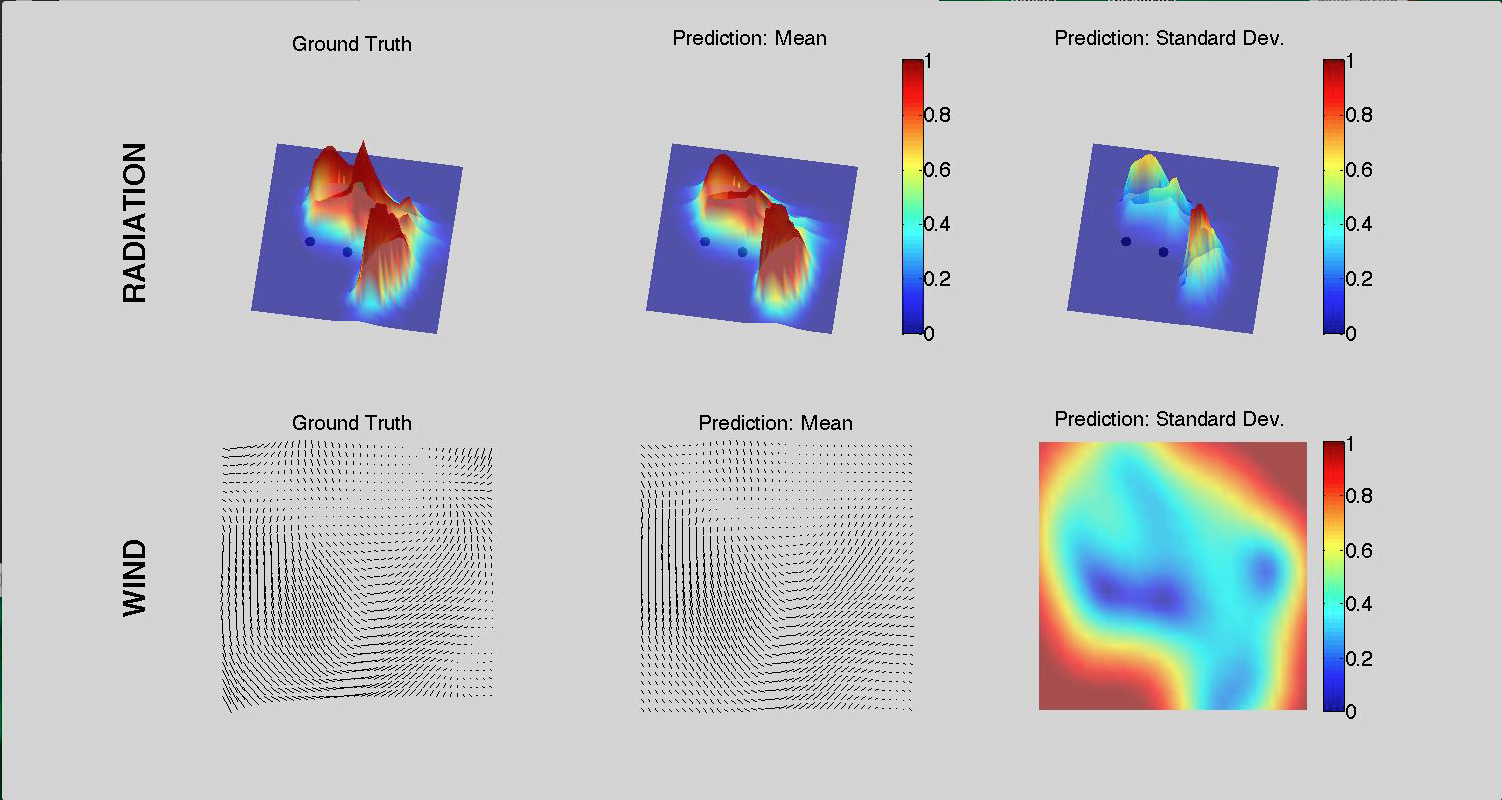
\includegraphics[width=0.45\textwidth]{figures/radiation_ss_calm.png}\\
%    (a) Slowly varying wind conditions\\ \ \\
%    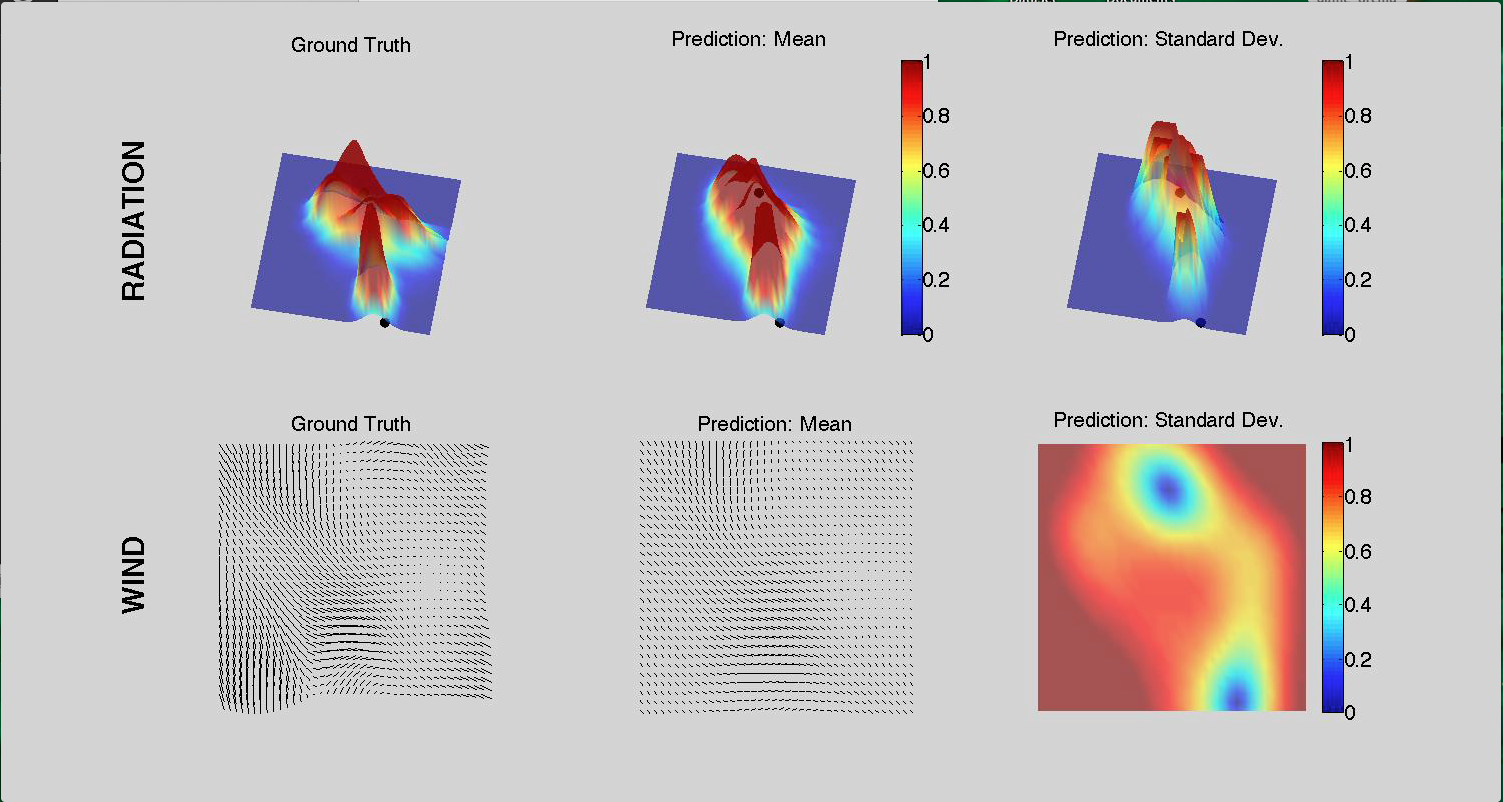
\includegraphics[width=0.45\textwidth]{figures/radiation_ss_gust.png}\\
%    (b) Gusty wind conditions 
%\caption{\label{radiation_screen_shots} Radiation and wind simulation ground truth and EKF estimates obtained using measurements from monitor agents (black dots).  Left most panes are ground truth radiation and wind conditions, the middle panes are corresponding estimates and right most panes are state uncertainties:  (a) Invariant and (b) gusty wind conditions.}
%\end{center}
%\end{figure}

\subsection{System architecture}
[Wenchao: adapt this to version 2.0] AtomicOrchid is based on the open-sourced geo-fencing game MapAttack\footnote{http://mapattack.org} that has been iteratively developed for a responsive, (relatively) scalable experience.  The location-based game is realized by client-server architecture, relying on real-time data streaming between client and server.

The client-server architecture is depicted in figure XX. Client-side requests for for less dynamic content use HTTP. Frequent events, such as location updates and radiation exposure, are streamed to clients to avoid the overhead of HTTP. In this way, field responders are kept informed in near real-time.

The planning agent agent ... [add implementation detail]

The platform is built using the geoloqi platform, Sinatra for Ruby, and state-of-the-art web technologies such as socket.io, node.js, redis and Synchrony for Sinatra, and the Google Maps API. Open source mobile client apps that are part native, part browser based exist for iPhone and Android; we adapted an Android app to build the mobile responder app.

\section{Real-world evaluation}
[Note: currently not sure whether to include the non-agent runs. Problematic because: a) unequal number of responders, b) HQ staffed by students in non-agent condition; researchers in agent-condition, c) not enough cases for a quantitative comparison anyways?.]
(\textbf{Joel: the population type does not matter so much for AAMAS as tar as I've seen. So go ahead with the analysis of the no-agent condition.})
We ran four sessions of AtomicOrchid with participants recruited from the local university to evaluate mixed-initiative coordination in a disaster response scenario. The following sections describe the participants, procedure, session configuration and methods used to collect and analyse quantitative and qualitative data.

\subsection{Participants}
A total of 29 participants (XX of them were female) were recruited through posters and emails, and reimbursed with 15 pounds for 1.5-2 hours of study. The majority were students of the local university. [Say something about their map reading skills?]

\subsection{Procedure}
The procedure consisted of 30 minutes of game play, and about 1 hour of pre-game briefing, consent forms and a short training session, and post-game group discussion and questionnaire. 

%Upon arrival in the HQ (set up in a meeting room at the local university), participants were briefed and asked to consent to participate. They were presented with a demographic questionnaire to record gender, occupation, experience of using smartphones and level of map navigation skills.

At the end of the briefing in which mission objectives and rules were outlined, responder roles were randomly assigned to all participants (fire-fighter, medic, transporter, soldier). HQ in the agent condition was staffed by a different member of the research team in each session in order to mimick an experienced HQ whilst avoiding the same person running HQ every time. 

Field responders were provided with a smartphone; HQ coordinators with a laptop. The team was given 5 minutes to discuss a common game strategy. (\textbf{Joel: where did the agent run ?})

Field responders were then accompanied to the starting point within the designated game area, about 1 minute walk from headquarters. Once field responders were ready to start, HQ sent a `game start' message. After 30 minutes of game play the field responders returned to the HQ for the post-game session, which consisted of a questionnaire aimed at collecting participants' feedback on (1) first impressions of the game; (2) usability of the system, and; (3) coordination issues in the game. A group interview was then conducted, before participants were debriefed and dismissed.

\subsection{Game sessions}
We ran two sessions without the planner agent, and two sessions with the planner agent to be able to compare team performance in the two conditions. We also ran a pilot study for each condition. The pilot study showed that this was a challenging, yet not too overwhelming number of targets to collect in a 30 min game session. There were four targets for each of the four target types.
The target locations, pattern of cloud movement and expansion were kept constant for all game sessions. 

The role allocation of the 8 field responders per session is depicted in table XX. One of the non-agent sessions only had 5 field responders due to drop outs. 

The terrain of the game area includes grassland, a lake, buildings, roads, and footpaths and lawns (see figure XX). There are two drop off zones and 16 targets.

\subsection{Methods}
We took a mixed methods approach to data collection and analysis. In addition to quantitative questionnaires, a semi-structured group interview was conducted that aimed at eliciting important decision points, strategies and the overall decision-making process. Furthermore, researchers with camcorders recorded the game play. One researcher recorded action in the HQ, and four other researchers each shadowed a field responder team with a camcorder.

We developed a log file replay tool to help with data analysis of time stamped system logs that contain a complete record of the game play, including responders' GPS location, their health status and radioactive exposure, messages, cloud location, locations of target objects and task status.

Video recordings of field action were catalogued to identify sequences (episodes) of interest (cf. Heath et al., 2010). Key decision points in teaming and task allocation served to index the episodes. Interesting distinct units of interaction were transcribed and triangulated with log files of relevant game activity for deeper analysis. Due to space constraints we can only  present one fragment in this paper to illustrate how human-agent collaboration typically unfolded (TODO).

How are remote messages used as a coordination resource? We use speech-act theory (Searle, 1975) to classify messages sent between and among responders and HQ. We focus on the most relevant types of acts in this paper (which are also the most frequently used in AtomicOrchid):

\begin{itemize}
\item Assertives: \textit{speech acts that commit a speaker to the truth of the expressed proposition}; these were a common category as they include messages that contain situational information.
\item Directives: \textit{speech acts that are meant to cause the hearer to take a particular action}, e.g. requests, commands and advice, including task and team allocation messages. 
\end{itemize}

\subsection{Results}

\paragraph{Structure}
\begin{itemize}
\item  \textit{Overall performance}. Draw on metrics below: tasks completed, number and categorisation of messages (only directives and assertives). 
\item \textit{Agent performance}. Metrics from below: Number of instructions sent, robustness etc. 
\item \textit{Task allocation}: How task allocation unfolded in the agent vs. non-agent condition. (Message handling (from JSCWS paper) vs. task handling diagram...) This is where we'd show a fragment to illustrate? -> Shows overall performance increase in performance
\item \textit{Rejecting tasks}: When and why did it happen? (-> pick this up in the discussion re. Gopal's/Feng's point on adjustable planning?). 
\item \textit{The role of HQ}: monitoring, supporting and dealing with contingencies. Some example messages. Draw on HQ metrics. (-> Shows division of labour and the benefits of human-agent collaboration).
\end{itemize} 
 
Joel and Wenchao
\begin{enumerate}
\item Explain setup of experiment - area of interest + setup of tasks
\item Explain evaluation = quantitative and qualitative.
\end{enumerate}
\paragraph{Metrics}
\begin{itemize}
\item{Comparisons between with/without agent versions for the below:}
\item{Performance of FR: number of tasks completed, time on task?, number of messages sent, number of teams formed and disbanded, time on team, acknowledgements of tasks}
\item{Messages: classification}
\item{Health}
\item{Distance travelled}
\item{HQ: number of agent monitoring actions (clicks), number of 'supporting'/related messages (e.g., enforcement, contradictions/overriding)}
\item{Agent performance: number of instructions, number of replanning steps, replanning robustness (diversion of task allocation compared to previous step)}
\item{Following instructions ('obedience'): number of instructions followed vs. not followed (incl. number of HQ interventions/overriding agent allocation), instruction handling diagram}
\item
\end{itemize}
